\mode*

% Since this a solution template for a generic talk, very little can
% be said about how it should be structured. However, the talk length
% of between 15min and 45min and the theme suggest that you stick to
% the following rules:  

% - Exactly two or three sections (other than the summary).
% - At *most* three subsections per section.
% - Talk about 30s to 2min per frame. So there should be between about
%   15 and 30 frames, all told.


\section{Multilateral säkerhet}
\begin{frame}{\insertsubsectionhead}
  \begin{quote}
    Privacy is a transient notion.
    It started when people stopped believing that God could see everything and 
    stopped when governments realised there was a vacancy to be filled.
  \end{quote}
  \begin{flushright}
    Roger Needham
  \end{flushright}
\end{frame}

\subsection{Gittermodellen (lattice model)}
\begin{frame}{\insertsubsectionhead}
  \begin{itemize}
    \item Vi kan även lägga till speciella kodord till klassificeringarna.
    \item En klassificering med ett eller flera kodord utgör en 
      \emph{säkerhetskategori (security category eller compartment)}.
    \item Detta ger multilateral säkerhet.
  \end{itemize}
\end{frame}

\begin{frame}{\insertsubsectionhead}
  \begin{figure}
    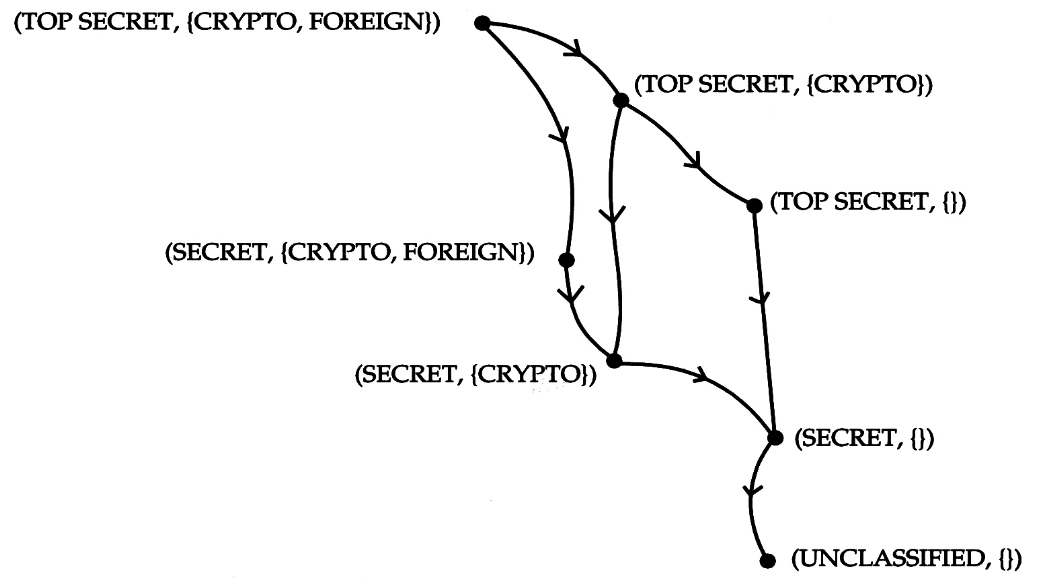
\includegraphics[height=0.7\textheight]{lattice.png}
    \caption{Exempel på gittermodellen, idén är att BLP bara behöver en 
    partiell ordning.}
  \end{figure}
\end{frame}

\subsection{Kinesiska muren-modellen}
\begin{frame}{\insertsubsectionhead}
  \begin{itemize}
    \item Utvecklades av Brewer och Nash.
    \item Har sitt ursprung hos bankerna.
    \item \emph{Separation of duty}: en användare får utföra \(A\) eller \(B\), 
      men inte båda.
    \item En systemadministratör får göra allt i ett system, men loggarna finns 
      hos någon annan systemadministratör.
  \end{itemize}
\end{frame}
\begin{frame}{\insertsubsectionhead}
  \begin{block}{Kinesiska muren}
    Låt \(c\) beteckna en resurs, \(y(c)\) är \(c\):s ägare och \(x(c)\) är 
    dess intressekonfliktklass.
    Då kan Kinesiska muren uttryckas enligt BLP som följande:
    \begin{description}
      \item[Simple security property] Ett subjekt \(s\) har tillgång till \(c\) 
        om och endast om för alla \(c^\prime\) som \(s\) kan \emph{läsa från} 
        gäller \(y(c)\notin x(c^\prime)\) eller \(y(c) = y(c^\prime)\).
      \item[*-property] Ett subjekt \(s\) kan skriva till \(c\) om och endast 
        om \(s\) inte kan läsa något \(c^\prime\) sådant att \(x(c^\prime)\neq 
        \emptyset\) och \(y(c)\neq y(c^\prime)\).
    \end{description}
  \end{block}
\end{frame}

\subsection{BMA-modellen}
\begin{frame}[allowframebreaks]{\insertsubsectionhead}
  \begin{itemize}
    \item Varje patientjournal har en åtkomstkontrollista (\emph{access control 
      list}, ACL) med alla som får läsa och skriva till journalen.
    \item För att komma åt journal:
      \begin{itemize}
        \item En läkare får öppna journalen med sig själv och patienten på 
          ACL:en.
        \item Vid remiss, en läkare får öppna journalen med sig själv, 
          patienten och remitterande läkare på ACL:en.
      \end{itemize}
    \item Ägare: en läkare är ansvarig och kontrollerar ACL.
    \item Notifiering: alla förändringar av ACL notifieras till och godkänns av 
      patienten.
    \item Beständighet: ingen kan ta bort data inom en förutbestämd tidsperiod.
    \item Loggning: all åtkomst till journalen noteras i den med subjektets 
      identitet, tid och datum.
    \item Informationsflöde: information från journal \(A\) får föras över till 
      journal \(B\) om och endast om \(B\):s ACL är en del av \(A\):s.
    \item Sammanställningskontroll: patienter ska få en särskild notifiering om 
      någon person med tillgång till en stor mängd patientjournaler föreslås 
      läggas till ACL:en.
    \item Trusted computing base: datorsystem som hanterar patientjournaler ska 
      påtvinga dessa principer.
  \end{itemize}
\end{frame}

\subsection{Inferenskontroll}
\begin{frame}{\insertsubsectionhead}
  \begin{itemize}
    \item Att avanonymisera statistik: Vad är medelbetyget för alla kvinnliga 
      studenter på Nätverksdriftsprogrammet i åk 1?
    \item Om det inte går: Vad är medelbetyget för alla studenter på 
      Nätverksdriftsprogrammet, och vad är medelbetyget för alla manliga 
      studenter på Nätverksdriftsprogrammet?
      \begin{itemize}
        \item Nu kan jag beräkna medelbetyget för våra kvinnliga deltagare.
      \end{itemize}
  \end{itemize}
\end{frame}


%%% REFERENCES %%%

\begin{frame}[allowframebreaks]
  \printbibliography
\end{frame}
